\documentclass[12pt]{amsart}
\usepackage{etex}
\usepackage{amsmath, psfrag}
\usepackage{amsfonts}
\usepackage{amsthm}
\usepackage{color}
\usepackage[final]{graphicx}
\usepackage[right=2cm, left=2cm, top=2cm, bottom=2cm]{geometry}

%%%%%WHAT WORKS FOR TEST TIKZ
\usepackage{tikz,adjustbox,pdfpages}
\usetikzlibrary{decorations.pathreplacing}

\usepackage[]{subfig,floatrow}
\floatsetup[table]{style=plaintop}
\floatsetup[figure]{valign=c, heightadjust=object,  framefit = yes}
\floatsetup[subfigure]{heightadjust=object, valign=c, framefit = yes}
\renewcommand\subfloatrowsep{\hskip  4\columnsep}
\newcommand{\spacebetween}{\vskip  12pt}
\usetikzlibrary{calc, through, shapes, positioning, decorations}
\tikzstyle{vertexb}=[shape=circle, draw=black, fill=black,inner sep=0pt,minimum size=4pt]
\tikzstyle{vertexr}=[shape=circle, draw=red, fill=red,inner sep=0pt,minimum size=3pt]
\tikzstyle{vertexg}=[shape=circle, draw=green, fill=green,inner sep=0pt,minimum size=3pt]
\tikzstyle{vertexgr}=[shape=circle, draw=black, fill=black!20,inner sep=0pt,minimum size=4pt]
\tikzstyle{vertexw}=[shape=circle, draw=black, fill=white,inner sep=0pt,minimum size=4pt]
\tikzstyle{vertex}=[circle, draw, inner sep=0pt, minimum size=6pt,fill=white]
%\tikzstyle{vertex}=[circle, draw, inner sep=1pt, minimum size=6pt,fill=black!20]
%%%%%%%%%%%%%%%%%%%%%%%
\renewcommand{\baselinestretch}{1.0}

\parskip .2in
\setcounter{page}{1} 
\pagenumbering{arabic}
\newtheorem{theorem}{Theorem}[section]
\newtheorem{thm}{{\bf Theorem}}[section]
\newtheorem{prop}{{\bf Proposition}}[section]
\newtheorem{cla}{{\bf Claim}}[section]
\newtheorem{lem}{{\bf Lemma}}[section]
\newtheorem{con}{{\bf Conjecture}}[section]
\newtheorem{cor}{{\bf Corollary}}[section]
\newtheorem{defi}{{\bf Definition}}[section]
\newtheorem{fact}{{\bf Fact}}[section]
\newtheorem{exm}{{\bf Example}}[section]
\newcommand{\lf}{\lfloor}
\newcommand{\lc}{\lceil}
\newcommand{\rf}{\rfloor}
\newcommand{\rc}{\rceil}
\newcommand{\s}{{\bf sat}}
\newcommand{\p}{{\bf SAT}}
\newcommand{\pl}{{\bf \underline{SAT}}}
\newcommand{\pu}{{\bf \overline{SAT}}}
\newtheorem{qes}{Question}%[section]
\newtheorem{pro}{Problem}%[section]
\newcommand{\rn}[1]{{\color{red} \bf #1}}
 
\definecolor{dark red}{HTML}{E41A1C}
\begin{document}


\title{Some Sample Graph Theory Pics using Tikz}
\date{\today}

\author[J. Faudree] {{\sl Jill Faudree} }
\address{Department of Mathematics and Statistics, University of Alaska Fairbanks, Fairbanks, AK 99775-6660}
\email{jrfaudree@alaska.edu}





\begin{abstract}
Some sample graph theory pictures using tikz. I will include more explanation later, but for now the reader will need to infer/guess/test.\end{abstract}
\maketitle


\section{Sample Pics}

\begin{figure}[ht!]
\begin{center}
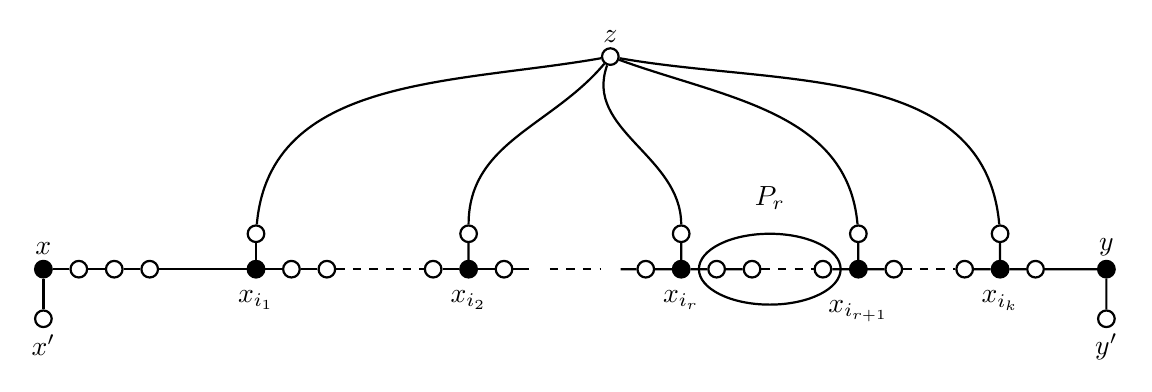
\begin{tikzpicture}[thick, scale=0.9]
\node (7) at (7,1){};\node (8) at (8,1){}; \node at (10.25,2) {$P_r$};
\tikzstyle{every node}=[vertex];
\node [minimum size=6pt, label=above:$x$, fill=black] (x) at (0,1){};
\node (01) at (0.5,1){}; \node (1) at (1,1){}; \node (21) at (1.5,1){};
\node [minimum size=6pt, label=below:$x_{i_1}$, fill=black] (xi1) at (3,1){};
\node (04) at (3.5,1){};\node (4) at (4,1){};\node (45) at (5.5,1){};
 \node (85) at (8.5,1){};
\node [minimum size=6pt, label=below:$x_{i_2}$, fill=black] (xi2) at (6,1){}; \node (6+) at (6.5,1){};
\node [minimum size=6pt, label=below:$x_{i_{r}}$, fill=black] (xr) at (9,1){}; \node (95) at (9.5,1){}; \node (10) at (10,1){};\node (xr2) at (9,1.5){};
 \node (11) at (11,1){};
\node [minimum size=6pt, label=below:$x_{i_{r+1}}$, fill=black] (xr+) at (11.5,1){};\node (12) at (12,1){}; \node (xr+2) at (11.5,1.5){};
\node (13) at (13,1){}; 
\node [minimum size=6pt, label=below:$x_{i_k}$, fill=black] (xik) at (13.5,1){};\node (14) at (14,1){};
\node [label=above:$y$, fill=black, minimum size=6pt] (y) at (15,1){};
\node [label=below:$x'$] (x1) at (0,0.3){};
\node [label=below:$y'$] (y1) at (15,0.3){};
\node [minimum size=6pt, label=above:$z$] (z) at (8,4){}; \node (n1) at (3,1.5){}; \node (n2) at (6,1.5){}; \node (nk) at (13.5,1.5){};
\draw (x1) -- (x) --(01)--(1)--(21)--(xi1)--(04)--(4) (45) -- (xi2) -- (6+)--(7);
\draw (8) -- (85)--(xr)--(95) -- (10) (11)--(12) (13) --(xik)--(14)-- (y)--(y1);
\draw  (n1) -- (xi1);
\draw [dashed] (4) -- (45) (7) -- (8) (10) -- (11) (12) -- (13);
\draw (z)to [out=190,in=85](n1);
\draw (z) to [out=230,in=90] (n2) (z) to [out=-10,in=95] (nk);
\draw (n2)--(xi2) (nk) -- (xik) (xr2) -- (xr) (xr+2) -- (xr+);
\draw (z) to [out=250,in=90] (xr2) (z) to [out=-20,in=95] (xr+2);
\draw (10.25,1) ellipse (1 and 0.5);
\end{tikzpicture}\end{center}
\caption{This figure illustrates the paths from vertex $z$ to $P$, a shortest path dominating a maximum number of vertices. Note the circled section denotes $P_r$, the section of the path strictly between two consecutive paths, $x_r$ and $x_{r+1}.$ }\label{firstill}
\end{figure}

Let $P_r=P(x_{i_r},x_{i_{r+1}})$ denote the subpath of $P$ strictly between two consecutive endpoints of paths from $z.$ (See Figure \ref{firstill}.)

\begin{figure}[ht!]
\begin{center}
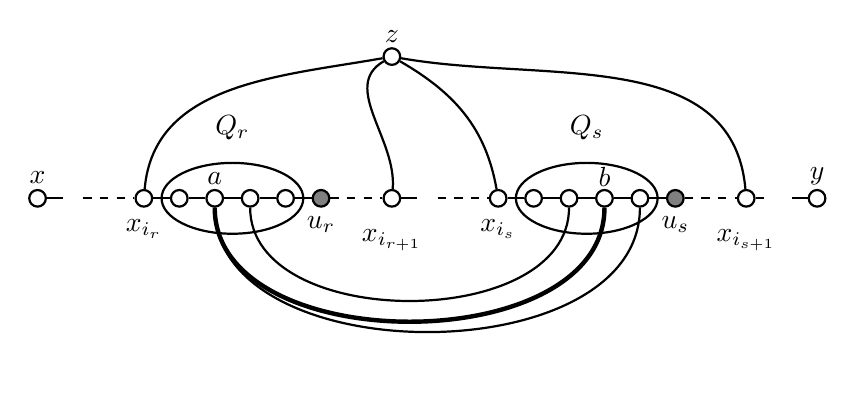
\begin{tikzpicture}[thick, scale=0.9]
\node (x+) at (0.5,0){}; \node at (2.75,1) {$Q_r$}; \node (xir++) at (5.5,0){}; \node at (7.75,1) {$Q_s$}; \node (y-) at (10.5,0){};
\node () at (,){};
\tikzstyle{every node}=[vertex];
\node [label=above:$x$] (x) at (0,0){};
\node [label=below:$x_{i_r}$] (xir) at (1.5,0){};
\node (r1) at (2,0){};\node [label=above:$a$](r2) at (2.5,0){};\node (r3) at (3,0){};\node (r4) at (3.5,0){};
\node [label=below:$u_r$,fill=black!50] (ur) at (4,0){};
\node [label=below:$x_{i_{r+1}}$] (xir+) at (5,0){};

\node [label=below:$x_{i_s}$] (xis) at (6.5,0){};
\node (s1) at (7,0){};\node (s2) at (7.5,0){};\node [label=above:$b$](s3) at (8,0){};\node (s4) at (8.5,0){};
\node [label=below:$u_s$,fill=black!50] (us) at (9,0){};
\node [label=below:$x_{i_{s+1}}$] (xis+) at (10,0){};
\node [label=above:$y$] (y) at (11,0){};

\node [label=above:$z$] (z) at (5,2){};

\draw (x) -- (x+) (xir)--(r1)--(r2)--(r3)--(r4)--(ur) (xir+)--(xir++);
\draw [dashed] (x+)--(xir) (ur)--(xir+);
\draw (2.75,0) ellipse (1 and 0.5);
\draw (xis)--(s1)--(s2)--(s3)--(s4)--(us) (y-)--(y);
\draw [dashed] (xir++)--(xis) (us)--(xis+)--(y-);
\draw (7.75,0) ellipse (1 and 0.5);
\draw (z)to [out=190,in=85](xir) (z)to [out=210,in=85](xir+) ;
\draw (z) to [out=-30,in=100](xis) (z)to [out=-10,in=95](xis+) ;
\draw [ultra thick] (r2) to [out=-90,in=-90] (s3);
\draw (r2) to [out=-90,in=-90] (s4);\draw (r3) to [out=-90,in=-90] (s2);
\end{tikzpicture}\end{center}
\caption{For each subpath of $P,$ $u_i$ is the first {\it{nonmovable}} vertex and, so,  those in $Q_i$ are all movable. Observe that any edges between distinct $Q_i$'s results in a path dominating more vertices by using the edge between vertices of smallest indices (or, alternatively, left-most vertices). New path: $x$ to $x_{i_r}$ to $z$ to $x_{i_s}$ to $a$ to $b$ to $y.$ Note that all vertices of $Q_r$ and $Q_s$ not on the new path are dominated elsewhere.}\label{secondill}
\end{figure}


\begin{figure}[ht!]
\begin{center}
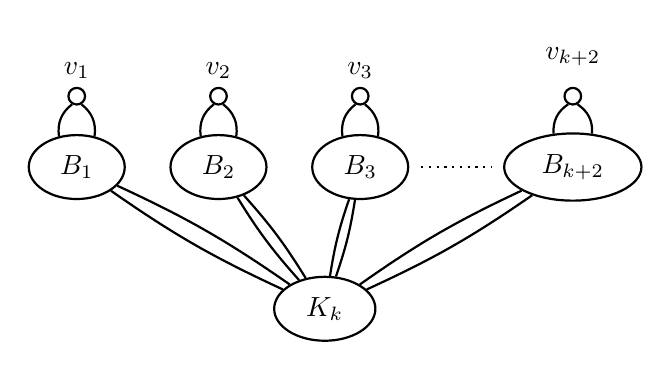
\begin{tikzpicture}[thick, scale=0.9]

\tikzstyle{every node}=[vertex];
\node[shape=ellipse, inner sep = 4pt, draw=black, fill=white] (kk) at (3.5,-2) {$\:K_k\:$};
\node[shape=ellipse, inner sep = 4pt, draw=black, fill=white] (b1) at (0,0) {$\:B_1\:$};
\node[shape=ellipse, inner sep = 4pt, draw=black, fill=white] (b2) at (2,0) {$\:B_2\:$};
\node[shape=ellipse, inner sep = 4pt, draw=black, fill=white] (b3) at (4,0) {$\:B_3\:$};
\node[shape=ellipse, inner sep = 4pt, draw=black, fill=white] (bk2) at (7,0) {$\:B_{k+2}\:$};
\node [label=above:$v_1$] (v1) at (0,1){};\node [label=above:$v_2$] (v2) at (2,1){};
\node [label=above:$v_3$] (v3) at (4,1){};\node [label=above:$v_{k+2}$] (vk2) at (7,1){};
\path (v1) edge [bend left = -30]  (b1);\path (v1) edge [bend right = -30]  (b1);
\path (v2) edge [bend left = -30]  (b2);\path (v2) edge [bend right = -30]  (b2);
\path (v3) edge [bend left = -30]  (b3);\path (v3) edge [bend right = -30]  (b3);
\path (vk2) edge [bend left = -30]  (bk2);\path (vk2) edge [bend right = -30]  (bk2);

\path (kk) edge [bend left =-5]  (bk2);\path (kk) edge [bend right = -5]  (bk2);
\path (kk) edge [bend left =-5]  (b1);\path (kk) edge [bend right = -5]  (b1);
\path (kk) edge [bend left =-5]  (b2);\path (kk) edge [bend right = -5]  (b2);
\path (kk) edge [bend left =-5]  (b3);\path (kk) edge [bend right = -5]  (b3);
\draw [dotted, shorten >=0.15cm,shorten <=.15cm] (b3)--(bk2);
\end{tikzpicture}\end{center}
\caption{Example \ref{ex1}}\label{example1}
\end{figure}

The following  corollary follows immediately from the statement of the theorem:




\begin{figure}[ht!]
\begin{center}
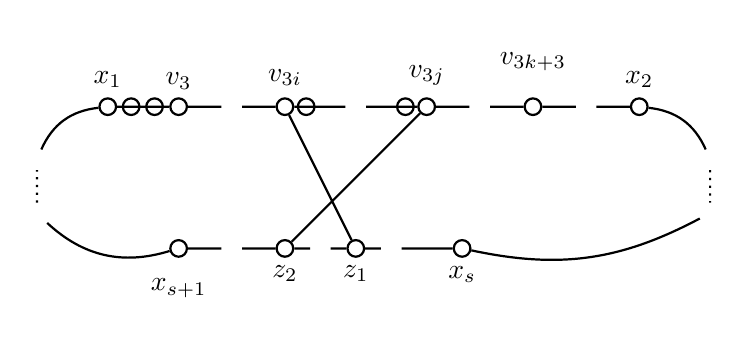
\begin{tikzpicture}[thick, scale=0.9]
\node (r1) at (8.5,-.75){}; \node (r2) at (8.5,-1.5){}; 
\node (l1) at (-1,-.75){}; \node (l2) at (-1,-1.5){}; 
\node (i1) at (1.75,0){};\node (i2) at (3.5,0){};\node (i3) at (5.25,0){};\node (i4) at (6.75,0){};
\node (i5) at (4,-2){};\node (i6) at (3,-2){};\node (i7) at (1.75,-2){};
\tikzstyle{every node}=[vertex];
\node [label=above:$x_1$] (x1) at (0,0){};
\node at (0.33,0){};\node at (0.66,0){};\node at (2.8,0){};\node at (4.2,0){};
\node [label=above:$v_3$] (v3) at (1,0){};
\node [label=above:$v_{3i}$] (v3i) at (2.5,0){};
\node [label=above:$v_{3j}$] (v3j) at (4.5,0){};
\node [label=above:$v_{3k+3}$] (v3k) at (6,0){};
\node [label=above:$x_2$] (x2) at (7.5,0){};
\node [label=below:$x_s$] (xs) at (5,-2){};
\node [label=below:$z_1$] (z1) at (3.5,-2){};
\node [label=below:$z_2$] (z2) at (2.5,-2){};
\node [label=below:$x_{s+1}$] (xs1) at (1,-2){};

\path (x2) edge [bend right = -30]  (r1);\path (r2) edge [bend right = -20]  (xs);
\path (xs1) edge [bend right = -30]  (l2);\path (l1) edge [bend right = -30]  (x1);
\draw [dotted] (r1) -- (r2) (l2)--(l1);
\draw (z2)--(v3j) (z1)--(v3i) (x1)--(v3)--(i1)--(v3i)--(i2)--(v3j)--(i3)--(v3k)--(i4)--(x2);
\draw (xs)--(i5)--(z1)--(i6)--(z2)--(i7)--(xs1);
\end{tikzpicture}\end{center}
\caption{A single pair of crossing edges results in a smaller cycle. Follow $x_1=v_0$ to $v_{3i}$, down to $z_1$, around to $v_{3j}$ via $x_s$, down to $z_2$ and back to $x_1.$}\label{pic:nocross}
\end{figure}


Now, using the previous upper and lower bounds on the number of excess chords, we produce the following contradiction: 
\begin{equation}\begin{split}\frac{1}{k+2}n&=\frac{(k+3)n}{k+2}-n\\
&\leq \frac{(k+3)n}{k+2}-(b+c+3k+7)\\
&<\frac{(k+3)n}{k+2}-b-2k-6-c\\
& \leq (2k+2)|X|\\
& = o(n).
\end{split}\end{equation} 





%% alg pic begins
\begin{table}
\caption{Cut-Set Selection Algorithm}
\label{alg}
\centering
\begin{tabular}{p{10cm}p{7cm}}
%interation 1
%\begin{figure}
\raisebox{-0.5\totalheight}{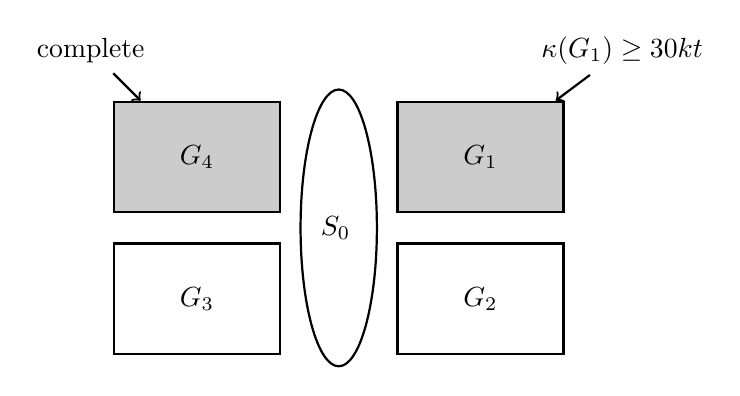
\begin{tikzpicture}[thick, scale=0.9]
\node[shape=ellipse, minimum height = 100pt, minimum width=4pt, draw=black, fill=white]  at (0,0) {$S_0\:$};
\node[shape=rectangle, minimum height = 40pt, minimum width=60pt, draw=black, fill=black!20] (g4) at (-2,1) {$G_4$};
\node[shape=rectangle, minimum height = 40pt, minimum width=60pt, draw=black, fill=white]  at (-2,-1) {$G_3$};
\node[shape=rectangle, minimum height = 40pt, minimum width=60pt, draw=black, fill=black!20]  (g1) at (2,1) {$G_1$};
\node[shape=rectangle, minimum height = 40pt, minimum width=60pt, draw=black, fill=white]  at (2,-1) {$G_2$};
\node (com) at (-3.5,2.5) {complete}; \node (con) at (4,2.5) {$\kappa(G_1)\geq 30kt$};
\draw [->] (com)--(g4); \draw [->](con) -- (g1);
\end{tikzpicture}}
%\end{figure}
& {Iteration 1: A minimum cut set $S_0$  results in four connected components, $G_1,\: G_2, \: G_3,$ and $G_4.$  So $\mathcal{S}=S_0$ and $k\leq s < t.$}\\ 
&\\
%iteration 2
%\begin{figure}
\raisebox{-.7\totalheight}{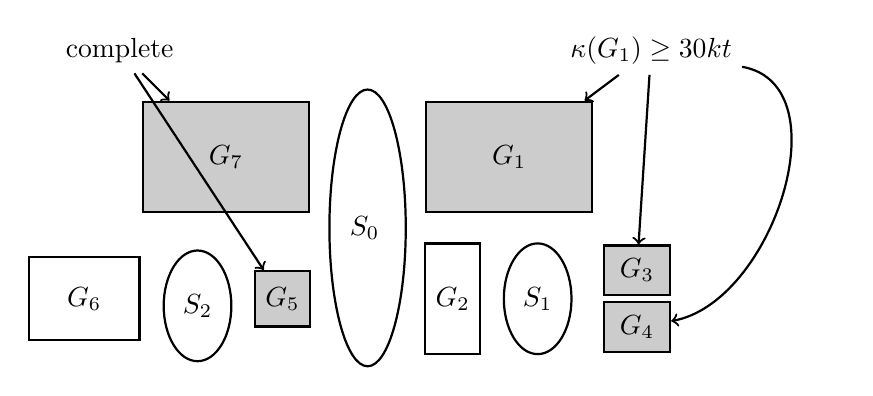
\begin{tikzpicture}[thick, scale=0.9]
\node[shape=ellipse, minimum height = 100pt, minimum width=4pt, draw=black, fill=white]  at (0,0) {$S_0\:$};
\node[shape=rectangle, minimum height = 40pt, minimum width=60pt, draw=black, fill=black!20] (g7) at (-2,1) {$G_7$};
\node[shape=rectangle, minimum height = 40pt, minimum width=60pt, draw=black, fill=black!20]  (g1) at (2,1) {$G_1$};
%split G_3
\node[shape=ellipse, minimum height = 40pt, draw=black, fill=white]  at (-2.4,-1.1) {$S_2$};
\node[shape=rectangle, minimum height = 30pt, minimum width=40pt, draw=black, fill=white] (g6) at (-4,-1) {$G_6$};
\node[shape=rectangle, minimum height = 20pt, minimum width=20pt, draw=black, fill=black!20] (g5) at (-1.2,-1) {$G_5$};
%split G_2
\node[shape=ellipse, minimum height = 40pt, draw=black, fill=white]  at (2.4,-1) {$S_1$};
\node[shape=rectangle, minimum height = 40pt, minimum width=20pt, draw=black, fill=white] (g2) at (1.2,-1) {$G_2$};
\node[shape=rectangle, minimum height = 18pt, minimum width=24pt, draw=black, fill=black!20] (g3) at (3.8,-.6) {$G_3$};
\node[shape=rectangle, minimum height = 18pt, minimum width=24pt, draw=black, fill=black!20] (g4) at (3.8,-1.4) {$G_4$};
%%
\node (com) at (-3.5,2.5) {complete}; \node (con) at (4,2.5) {$\kappa(G_1)\geq 30kt$};
\draw [->] (com)--(g7);\draw [->] (com)--(g5); \draw [->](con) -- (g1);\draw [->](con) -- (g3);
\draw [->](con) to[out=-10,in=10] (g4);
\end{tikzpicture}}
%\end{figure}
&{Iteration 2: Minimum cut sets $S_1$ and $S_2$ are found in noncomplete components of $G-\mathcal{S}$ with connectivity less than $30kt.$ Now,  $\mathcal{S}=S_0\cup S_1 \cup S_2 ,$  $s < t+2(30kt)$ and $G-\mathcal{S}$  results in seven connected components.}\\ 
&\\
%iteration 3
%\begin{figure}
\raisebox{-.8\totalheight}{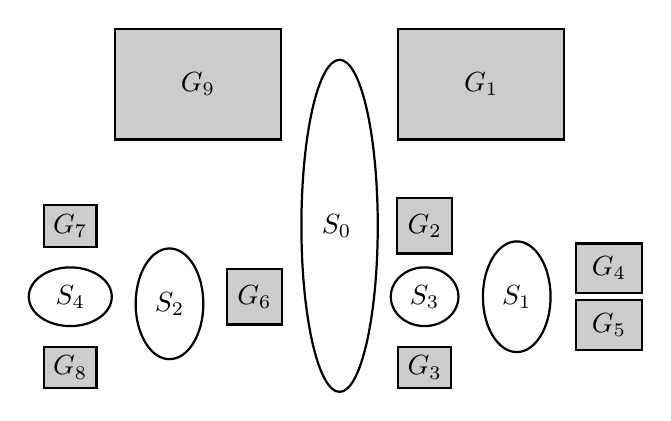
\begin{tikzpicture}[thick, scale=0.9]
\node[shape=ellipse, minimum height = 120pt, minimum width=4pt, draw=black, fill=white]  at (0,0) {$S_0\:$};
\node[shape=rectangle, minimum height = 40pt, minimum width=60pt, draw=black, fill=black!20] (g9) at (-2,2) {$G_9$};
\node[shape=rectangle, minimum height = 40pt, minimum width=60pt, draw=black, fill=black!20]  (g1) at (2,2) {$G_1$};
\node[shape=ellipse, minimum height = 40pt, draw=black, fill=white]  at (-2.4,-1.1) {$S_2$};
%split G_6
\node[shape=ellipse, minimum width = 30pt,  draw=black, fill=white] (s4) at (-3.8,-1) {$S_4$};
\node[shape=rectangle, minimum height = 10pt, minimum width=10pt, draw=black, fill=black!20] (g7) at (-3.8,0) {$G_7$};
\node[shape=rectangle, minimum height = 10pt, minimum width=10pt, draw=black, fill=black!20] (g8) at (-3.8,-2) {$G_8$};
%
\node[shape=rectangle, minimum height = 20pt, minimum width=20pt, draw=black, fill=black!20] (g6) at (-1.2,-1) {$G_6$};
\node[shape=ellipse, minimum height = 40pt, draw=black, fill=white]  at (2.5,-1) {$S_1$};
%spit G_2
\node[shape=ellipse, minimum width = 20pt, draw=black, fill=white] (s3) at (1.2,-1) {$S_3$};
\node[shape=rectangle, minimum height = 20pt, minimum width=20pt, draw=black, fill=black!20] (g2) at (1.2,0) {$G_2$};
\node[shape=rectangle, minimum height = 10pt, minimum width=10pt, draw=black, fill=black!20] (g3) at (1.2,-2) {$G_3$};
%
\node[shape=rectangle, minimum height = 18pt, minimum width=24pt, draw=black, fill=black!20] (g4) at (3.8,-.6) {$G_4$};
\node[shape=rectangle, minimum height = 18pt, minimum width=24pt, draw=black, fill=black!20] (g5) at (3.8,-1.4) {$G_5$};
\end{tikzpicture}}
%\end{figure}
& {Iteration 3: Minimum cut sets $S_3$ and $S_4$ are found in noncomplete components of $G-\mathcal{S}$ with connectivity less than $30kt.$ Now,  $\mathcal{S}=\cup_{i=0}^4 S_i ,$  $s < t+4(30kt)$ and $G-\mathcal{S}$  results in 9 connected components. The algorithm would terminate with all components either complete or with connectivity at least $30kt.$}\\
 & \\
\end{tabular}
\end{table} %%alg pic ends




Now, for $n$ sufficiently large, 
\begin{equation}\label{Gj_sig2} \begin{split}
\sigma_2(G_{j_1})&\geq \frac{2n}{k+2}+f(k)-2s \geq \frac{2|V(G_{j_1})| +2(n-|V(G_{j_1})|)}{k+2}+f(k)-2s\\
&> \frac{2|V(G_{j_1})|}{k+2} + \frac{2(\sigma_2(G)/2)}{k+2}-2s=\frac{2|V(G_{j_1})|}{k+2} + \frac{2n}{(k+2)^2}-2s\\
&>\frac{2|V(G_{j_1})|}{k+2}
\end{split}\end{equation} 
since $s=o(n).$

Because the steps used in Case 1 will be essentially the same in Cases 2 and 3, the steps are given names for ease of reference later. To aid the reader, pictures of the various steps are shown in Table \ref{cartoon}.

\begin{table}
\caption{Cartoon Illustrating the Proof of Theorem \ref{sigma2_shortpath}}
\label{cartoon}
\centering
\begin{tabular}{p{5cm}p{5cm}p{8cm}}
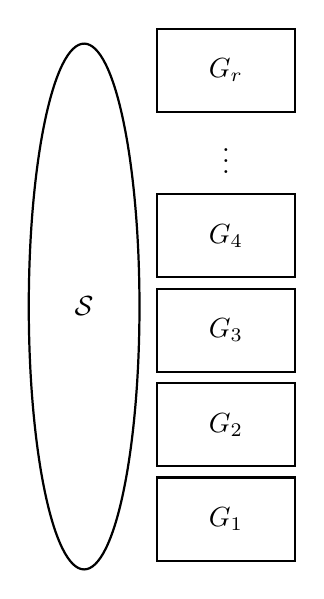
\begin{tikzpicture}[thick, scale=0.6]
\node[shape=ellipse, minimum height = 190pt, minimum width=40pt, draw=black, fill=white]  at (0,6.5) {$\:\mathcal{S}\:$};
\foreach \i in {1,...,4}{
	\node[shape=rectangle, minimum height = 30pt, minimum width=50pt, draw=black, fill=white] (g\i) at (3,2*\i) {$G_{\i}$};
}
\node[shape=rectangle, minimum height = 30pt, minimum width=50pt, draw=black, fill=white] (gr) at (3,11.5) {$G_r$};
\node[shape=rectangle,  draw=white, fill=white] (dots) at (3,9.75) {$\vdots$};
\end{tikzpicture}
&
% just G' 
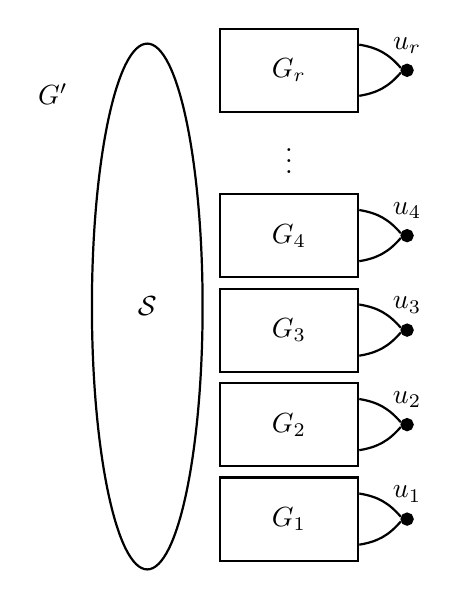
\begin{tikzpicture}[thick, scale=0.6]
\node[shape=ellipse, minimum height = 190pt, minimum width=40pt, draw=black, fill=white]  at (0,6.5) {$\:\mathcal{S}\:$};
\foreach \i in {1,...,4}{
	\node[shape=rectangle, minimum height = 30pt, minimum width=50pt, 		draw=black, fill=white] (g\i) at (3,2*\i) {$G_{\i}$};
	\node[shape=circle, draw=black, fill=black,inner sep=0pt,minimum size=4pt, label=$u_{\i}$] (u\i) at (5.5, 2*\i){};
	\path (u\i) edge [bend right = -20]  (g\i);\path (u\i) edge [bend left= -20]  (g\i);
}
\node[shape=rectangle, minimum height = 30pt, minimum width=50pt, draw=black, fill=white] (gr) at (3,11.5) {$G_r$};
\node[shape=circle, draw=black, fill=black,inner sep=0pt,minimum size=4pt, label=$u_{r}$] (ur) at (5.5,11.5){};
\path (ur) edge [bend right = -20]  (gr);\path (ur) edge [bend left= -20]  (gr);
\node[shape=rectangle,  draw=white, fill=white] (dots) at (3,9.75) {$\vdots$};
\node[shape=rectangle,  draw=white, fill=white] (G2) at (-2,11) {$G'$};
\end{tikzpicture}
&
%  G' and C'
\hspace{1.5cm}
\resizebox{5cm}{!}{%
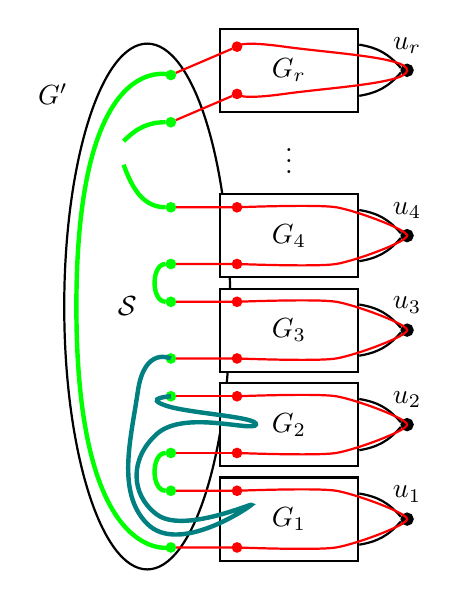
\begin{tikzpicture}[thick,scale=0.6]
\node[shape=ellipse, minimum height = 190pt, minimum width=60pt, draw=black, fill=white]  at (0,6.5) {$\:\mathcal{S}\hspace{.2in}\:$};
\foreach \i in {1,...,4}{
	\node[shape=rectangle, minimum height = 30pt, minimum width=50pt, draw=black, fill=white] (g\i) at (3,2*\i) {$G_{\i}$};
	\node[shape=circle, draw=black, fill=black,inner sep=0pt,minimum size=4pt, label=$u_{\i}$] (u\i) at (5.5, 2*\i){};
	\path (u\i) edge [bend right = -20]  (g\i);\path (u\i) edge [bend left= -20]  (g\i);
}
\node[shape=rectangle, minimum height = 30pt, minimum width=50pt, draw=black, fill=white] (gr) at (3,11.5) {$G_r$};
\node[shape=circle, draw=black, fill=black,inner sep=0pt,minimum size=4pt, label=$u_{r}$] (ur) at (5.5,11.5){};
\path (ur) edge [bend right = -20]  (gr);\path (ur) edge [bend left= -20]  (gr);
\node[draw=white, fill=white] (dots) at (3,9.75) {$\vdots$};
\node[draw=white, fill=white] (G2) at (-2,11) {$G'$};
%cycle
\foreach \i in {1,...,4}{
\node (b\i) at (4, 2*\i+0.6 ){};\node (d\i) at (4, 2*\i - 0.6 ){};
}
\tikzstyle{every node}=[vertexg];
\node (wr) at (0.5,11.4){}; \node (zr) at (0.5, 10.4){};
\foreach \i in {1,...,4}{
\node (w\i) at (0.5, 2*\i +0.6){};\node (z\i) at (0.5, 2*\i - 0.6 ){};
}
\tikzstyle{every node}=[vertexr];

\node (ar) at (1.9, 12 ){};\node (cr) at (1.9, 11){};
\draw [red] plot [smooth, tension = 1] coordinates {(cr) (2.9,11) (ur) (2.9,12) (ar)};
\draw [red] (wr) -- (ar) (zr) -- (cr);
\foreach \i in {1,...,4}{
\node (a\i) at (1.9, 2*\i +0.6 ){};
\node (c\i) at (1.9, 2*\i -0.6){};
\draw [red] plot [smooth, tension = 0.4] coordinates {(c\i)(d\i)(u\i)(b\i)(a\i)};
\draw [red] (w\i) -- (a\i) (z\i) -- (c\i);
}
\draw [green, ultra thick] (w1) to [out=180, in=180] (z2);
\draw [teal, ultra thick] plot [smooth, tension = 1] coordinates {(0.5,4.6) (0.4, 4.4) (2.3,4)  (0.2,3.8) (0.2,2.1) (2.2,2.3) (0,1.9) (-.2,4.7) (0.5,5.4)};
\draw [green, ultra thick] (w3) to [out=180, in=180] (z4) (w4) to [out=180, in=-70] (-.5,9.5);
\draw [green, ultra thick] plot [smooth, tension = 2] coordinates { (z1) (-1.5,6.5) (wr)};
\draw [green, ultra thick] (zr) to [out=180 , in= 45] (-.5,10) ;
\end{tikzpicture}}\\
This shows $\mathcal{S}$ and the components of $G-\mathcal{S}$
&
This shows $G'$ with added vertices $u_i.$
&
This shows $C'$ (in red, green, and teal) in $G'$. Note that the the $Q_i'$s are depicted in green (and teal) which is the portion of $C'$ left intact. The teal section ($Q_3'$) illustrates how complicated these connector sections may be. They may include vertices from $G$ outside $\mathcal{S}$ and possibly vertices from $T.$ \\
&&\\
\end{tabular} 
%\end{table}     

%\begin{table}

%\label{cartoon2}
%\centering
\begin{tabular}{p{9cm}p{9cm}}
%  G with T_i identified
\hspace{1.5cm}
\resizebox{5cm}{!}{%
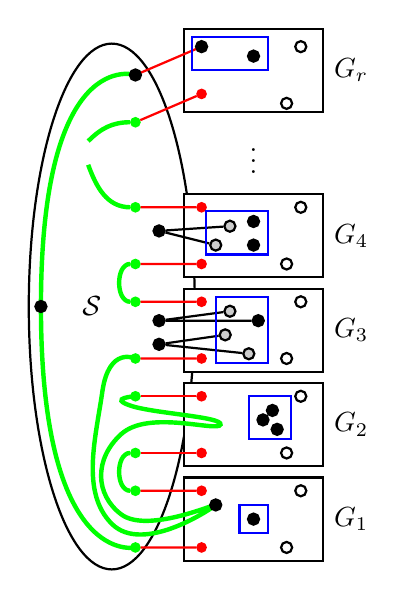
\begin{tikzpicture}[thick,scale=0.6]
\node[shape=ellipse, minimum height = 190pt, minimum width=60pt, draw=black, fill=white]  at (0,6.5) {$\:\mathcal{S}\hspace{.2in}\:$};
\foreach \i in {1,...,4}{
	\node[shape=rectangle, minimum height = 30pt, minimum width=50pt, draw=black, fill=white, label = right:{$G_{\i}$} ] (g\i) at (3,2*\i) {};
}
\node[shape=rectangle, minimum height = 30pt, minimum width=50pt, draw=black, fill=white, label = right:{$G_{r}$} ] (gr) at (3,11.5) {};
\node[draw=white, fill=white] (dots) at (3,9.75) {$\vdots$};
%Q_i'
\tikzstyle{every node}=[vertexg];
\node (wr) at (0.5,11.4){}; \node (zr) at (0.5, 10.4){};
\foreach \i in {1,...,4}{
\node (w\i) at (0.5, 2*\i +0.6){};\node (z\i) at (0.5, 2*\i - 0.6 ){};
}
\tikzstyle{every node}=[vertexr];
\node (ar) at (1.9, 12 ){};\node (cr) at (1.9, 11){};
\draw [red] (wr) -- (ar) (zr) -- (cr);
\foreach \i in {1,...,4}{
\node (a\i) at (1.9, 2*\i +0.6 ){};
\node (c\i) at (1.9, 2*\i -0.6){};
\draw [red] (w\i) -- (a\i) (z\i) -- (c\i);
}
\draw [green, ultra thick] (w1) to [out=180, in=180] (z2);
\draw [green, ultra thick] plot [smooth, tension = 1] coordinates {(0.5,4.6) (0.4, 4.4) (2.3,4)  (0.2,3.8) (0.2,2.1) (2.2,2.3) (0,1.9) (-.2,4.7) (0.5,5.4)};
\draw [green, ultra thick] (w3) to [out=180, in=180] (z4) (w4) to [out=180, in=-70] (-.5,9.5);
\draw [green, ultra thick] plot [smooth, tension = 2] coordinates { (z1) (-1.5,6.5) (wr)};
\draw [green, ultra thick] (zr) to [out=180 , in= 45] (-.5,10);
%black verts (T)
\tikzstyle{every node}=[vertexb];
\node at (wr){}; \node (g4inb) at (3,8.3){}; \node at (3,7.8){}; \node (g4out) at (1,8.1){}; \node (g3in2) at (3.1,6.2){};
\node (g1in) at (3,2){}; \node (g3out1) at (1,6.2){}; \node (g3out2) at (1, 5.7){}; \node at (ar){}; \node at (2.2,2.3){}; \node (grin) at (3,11.8){};
\node (g2in1) at (3.2,4.1){}; \node at (3.4,4.3){}; \node (g2in2) at (3.5,3.9){};
\node at (-1.5,6.5){};
%gray verts (nbhs of T)
\tikzstyle{every node}=[vertexgr];
\node (g4in1) at (2.5,8.2){}; \node (g4in2) at (2.2,7.8){};
\draw (g4in1) -- (g4out) -- (g4in2); 
\node (g3in1) at (2.5,6.4){};\node (g3in3) at (2.4,5.9){};\node (g3in4) at (2.9,5.5){};
\draw (g3in1) -- (g3out1) -- (g3in2) (g3in3) -- (g3out2) -- (g3in4);
%white verts (neither)
\tikzstyle{every node}=[vertexw];
\foreach \i in {1,...,4,5.7}{
\node at (4,2*\i+0.6){}; \node at (3.7,2*\i-0.6){}; 
}
% T_i boxes
\draw [blue,thick] ($(ar.north west)+(-0.13,0.13)$)  rectangle ($(grin.south east)+(0.2,-0.2)$);
\draw [blue,thick] ($(g4inb.north east)+(0.2,0.12)$)  rectangle ($(g4in2.south west)+(-0.1,-0.1)$);
\draw [blue,thick] ($(g3in1.north west)+(-0.2,0.2)$)  rectangle ($(g3in4.south east)+(0.3,-0.1)$);
\draw [blue,thick] ($(g2in1.north west)+(-0.2,0.4)$)  rectangle ($(g2in2.south east)+(0.2,-0.1)$);
\draw [blue,thick] ($(g1in.north west)+(-0.2,0.2)$)  rectangle ($(g1in.south east)+(0.2,-0.2)$);
\end{tikzpicture}}
&
\hspace{1cm}
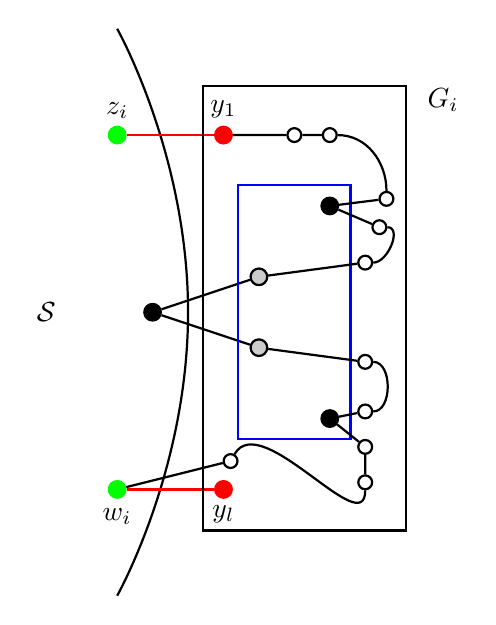
\begin{tikzpicture}[thick, scale=0.9]
\node at (4.6,3){$G_i$};
\draw [black] plot [smooth, tension = 1] coordinates {(0,4)(1,0)(0,-4)};
\node at (-1,0){$\mathcal{S}$};
\tikzstyle{every node}=[vertexg];
\node [minimum size = 6pt,label=above:{$z_i$}](zi) at (0,2.5){};
\node [minimum size = 6pt,label=below:{$w_i$}](wi) at (0,-2.5){};
\tikzstyle{every node}=[vertexr];
\node [minimum size = 6pt,label=above:{$y_1$}](y1) at (1.5,2.5){};
\node [minimum size = 6pt,label=below:{$y_l$}](yl) at (1.5,-2.5){};
\draw [red] (zi) -- (y1) (yl) -- (wi);
\tikzstyle{every node}=[vertexb];
\node [minimum size = 6pt](tout) at (.5,0){};
\node [minimum size = 6pt](tin1) at (3,1.5){};\node [minimum size = 6pt](tin2) at (3,-1.5){};
\tikzstyle{every node}=[vertexgr];
\node  [minimum size = 6pt](tout1) at (2,0.5){};
\node  [minimum size = 6pt](tout2) at (2,-0.5){};
\draw (tout1) -- (tout) -- (tout2);
\draw [blue,thick] ($(tout1.north west)+(-0.2,1.2)$)  rectangle ($(tin2.south east)+(0.2,-0.2)$);
\tikzstyle{every node}=[vertexw];
\node [minimum size = 5pt] (v11) at (2.5,2.5){}; \node [minimum size = 5pt](v12) at (3,2.5){};\node [minimum size = 5pt](v13) at (3.8,1.6){};
\node [minimum size = 5pt](v21) at (3.7,1.2){};\node [minimum size = 5pt](v22) at (3.5,.7){};
\node [minimum size = 5pt](v31) at (3.5,-.7){};\node [minimum size = 5pt](v32) at (3.5,-1.4){};
\node [minimum size = 5pt](v41) at (3.5,-1.9){};\node [minimum size = 5pt](v42) at (3.5,-2.4){};\node [minimum size = 5pt](v43) at (1.6,-2.1){};
\draw (y1) -- (v11) -- (v12) to [out=0,in=90] (v13);
\draw (v13) -- (tin1) -- (v21) (v22) -- (tout1) (tout2) -- (v31) (v32) -- (tin2) -- (v41) -- (v42) (v43) -- (wi);
\draw (v21) to [out=0, in =0] (v22);\draw (v31) to [out=0, in =0] (v32);
\draw (v42) to [out=-90, in =60] (v43);
\draw [black,thick] ($(y1.north west)+(-0.2,.6)$)  rectangle ($(v42.south east)+(0.5,-0.6)$);

\end{tikzpicture}
\\
In the diagram above, black vertices are in $T$, gray vertices are designated neighbors of vertices of $T_{\mathcal{S}}$ not on any green path. For each $G_i$, the set $T_i$ is in a blue box. Observe that vertices of $T$ on any $Q_j'$ (in green) are not included in any $T_i$.
&
This diagram illustrates how the red portion of $C'$ is replaced with a path containing the vertices of $T_i.$ As before, vertices of $T$ are black, associated neighbors of vertices that belong to $G_i$ are in gray. Observe that $y_1$ and $y_l$ may or may not be on this new path. It is enough to know that $z_i$ and $w_i$ have distinct neighbors in $G_i.$
\\
\end{tabular} \end{table}

\begin{theorem} [Tur\'an, '40]  If $3 \leq p \leq n$, then \textbf{ex}$(n, K_p ) =\left(1-\frac{1}{p-1 }\right) \frac{n^2}{2} $  and the unique $K_p$ -saturated 
graph of size \textbf{ex}$(n, K_p )$ is the balanced (or nearly balanced) complete $(p-1)$-partite graph. \end{theorem}

\begin{tabular}{p{6cm}rr}
The unique $K_5$-free graph with \textbf{ex}$(13,K_5)$ edges& \quad\quad&
\adjustbox{valign=c}{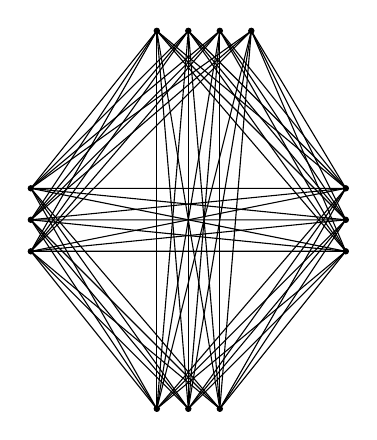
\begin{tikzpicture}[scale=0.4]
     \node[draw, fill=black, circle, scale=0.2] (d4) at (7,8) {};
     \foreach \number in {1,...,3}{
	\node[draw, fill=black, circle, scale=0.2] (a\number) at (0,\number) {};
	\node[draw, fill=black, circle, scale=0.2] (b\number) at (10,\number) {};
	\node[draw, fill=black, circle, scale=0.2] (c\number) at (3+\number,-4) {};
	\node[draw, fill=black, circle, scale=0.2] (d\number) at (3+\number,8) {};
	};
   \foreach \num in {1,2,3,4}{
   	\foreach \mur in {1,2,3}{
        \draw (d\num) -- (a\mur);
         \draw (d\num) -- (b\mur);
          \draw (d\num) -- (c\mur);
   }}
   \foreach \num in {1,2,3}{
   	\foreach \mur in {1,2,3}{
        \draw (c\num) -- (a\mur) -- (b\num);
        \draw (c\num) -- (b\mur);
   }}
    \end{tikzpicture}}
\end{tabular}



\begin{tabular}{p{6cm}rr}
The unique $K_5$-free graph with \textbf{sat}$(13,K_5)$ edges& \quad\quad&
\adjustbox{valign=c}{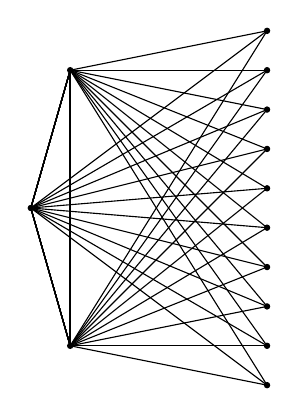
\begin{tikzpicture}[scale=0.5]
      \node[draw, fill=black, circle, scale=0.2] (a) at (0,5.5) {};
      \node[draw, fill=black, circle, scale=0.2] (b) at (1,2) {};
     \node[draw, fill=black, circle, scale=0.2] (c) at (1,9) {};
     \foreach \number in {1,...,10}{
	\node[draw, fill=black, circle, scale=0.2] (\number) at (6,\number) {};
	\draw (a) -- (\number); \draw (b) -- (\number); \draw (c) -- (\number);
	\draw (a) -- (b) -- (c) -- (a);
	};
    \end{tikzpicture}}
\end{tabular}

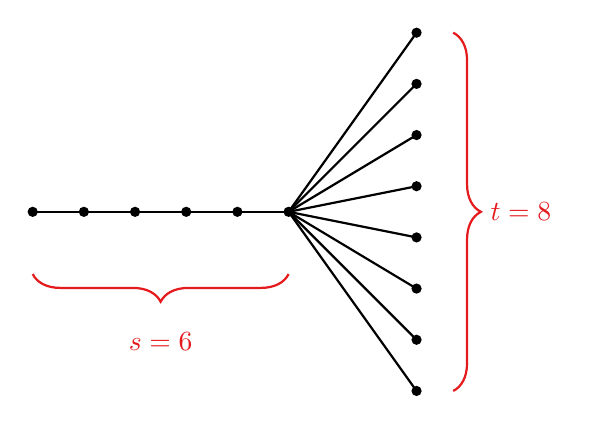
\begin{tikzpicture}[thick, scale=0.65]
     \foreach \number in {1,...,6}{
	\node[draw, fill=black, circle, scale=0.3] (\number) at (\number,4.5) {};
	};
    \draw (1) -- (6);
     \foreach \number in {1,...,8}{
	\node[draw, fill=black, circle, scale=0.3] (b\number) at (8.5,\number) {};
	\draw (6) -- (b\number);
	};
	\draw [decorate,dark red, decoration={brace,amplitude=10pt,mirror,raise=4pt},yshift=0pt]
(9,1) -- (9,8) node [dark red,midway, xshift=1cm] {
$t=8$};
\draw [decorate,dark red, decoration={brace,amplitude=10pt,mirror,raise=4pt},yshift=0pt]
(1,3.5) -- (6,3.5) node [dark red,midway, yshift=-1cm] {
$s=6$};
    \end{tikzpicture} 
    
    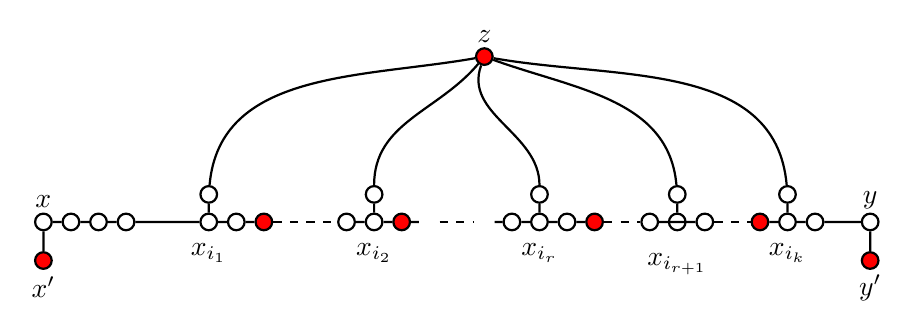
\begin{tikzpicture}[thick, scale=0.7]
\node (7) at (7,1){};\node (8) at (8,1){}; 
%\node at (10.25,2) {$P_r$};
\tikzstyle{every node}=[vertex];
\node [minimum size=6pt, label=above:$x$] (x) at (0,1){};
\node (01) at (0.5,1){}; \node (1) at (1,1){}; \node (21) at (1.5,1){};
\node [minimum size=6pt, label=below:$x_{i_1}$] (xi1) at (3,1){};
\node (04) at (3.5,1){};\node [fill=red] (4) at (4,1){};\node (45) at (5.5,1){};
 \node (85) at (8.5,1){};
\node [minimum size=6pt, label=below:$x_{i_2}$] (xi2) at (6,1){}; \node [fill=red] (6+) at (6.5,1){};
\node [minimum size=6pt, label=below:$x_{i_{r}}$] (xr) at (9,1){}; \node (95) at (9.5,1){}; \node [fill=red](10) at (10,1){};\node (xr2) at (9,1.5){};
 \node (11) at (11,1){};
\node [minimum size=6pt, label=below:$x_{i_{r+1}}$] (xr+) at (11.5,1){};\node (12) at (12,1){}; \node  (xr+2) at (11.5,1.5){};
\node [fill=red] (13) at (13,1){}; 
\node [minimum size=6pt, label=below:$x_{i_k}$] (xik) at (13.5,1){};\node (14) at (14,1){};
\node [label=above:$y$, minimum size=6pt] (y) at (15,1){};
\node [label=below:$x'$, fill=red] (x1) at (0,0.3){};
\node [label=below:$y'$, fill=red] (y1) at (15,0.3){};
\node [minimum size=6pt, label=above:$z$, fill=red] (z) at (8,4){}; \node (n1) at (3,1.5){}; \node (n2) at (6,1.5){}; \node (nk) at (13.5,1.5){};
\draw (x1) -- (x) --(01)--(1)--(21)--(xi1)--(04)--(4) (45) -- (xi2) -- (6+)--(7);
\draw (8) -- (85)--(xr)--(95) -- (10) (11)--(12) (13) --(xik)--(14)-- (y)--(y1);
\draw  (n1) -- (xi1);
\draw [dashed] (4) -- (45) (7) -- (8) (10) -- (11) (12) -- (13);
\draw (z)to [out=190,in=85](n1);
\draw (z) to [out=230,in=90] (n2) (z) to [out=-10,in=95] (nk);
\draw (n2)--(xi2) (nk) -- (xik) (xr2) -- (xr) (xr+2) -- (xr+);
\draw (z) to [out=250,in=90] (xr2) (z) to [out=-20,in=95] (xr+2);
%\draw (10.25,1) ellipse (1 and 0.5);
\end{tikzpicture}

%%%BIBLIOGRAPHY%%%
\begin{thebibliography}{99}

\bibitem[AS]{as} N. Alon,  J. Spencer,  {\bf The probabilistic method} Third edition. Wiley-Interscience Series in Discrete Mathematics and Optimization. John Wiley \& Sons, Inc., Hoboken, NJ, 2008. xviii+352 pp. ISBN: 978-0-470-17020-5 

\bibitem[VA74]{va74} V. Arnautov, Estimation of the exterior stability number of a graph by means of the minimal degree of the vertices (Russian), {\it{Prikl. Mat. I Programmirovanie}} 11 (1974), 3-8, 126. 

\bibitem[JB80]{jb80} J. Bondy, Longest paths and cycles in graphs of high degree, Research Report CORR 80-16, Univ. of Waterloo, Waterloo, Ontario (1980).

\bibitem [BF87]{bf87} J. Bondy, G. Fan,
A sufficient condition for dominating cycles
{\it{Discrete Math.}} 67 (1987), no. 2, 205-208. 

\bibitem[HB88]{b88} H. Broersma, Existence of $\Delta_\gamma$-cycles and $\Delta_\gamma$-paths, {\it J. Graph Theory} 12 (1988), 499-507.

\bibitem[CFHJL]{cfhjl} G. Chen, M. Ferrara, Z. Hu, M. Jacoboson, H. Liu, Degree conditions for spanning brooms, {\it{J. Graph Theory}}, 77 (2014), no. 3, 237-250.

\bibitem[CCE]{cce85} B. Clark, C. Colbourn, P. Erd\H{o}s, A conjecture on dominating cycles, {\it{Comb. graph theory and computing}}, Proc. 16th Southeast Conf., Boca Raton/Fla. 1985, Cong. Numerantium 47, 189-197 (1985).

\bibitem [GD52]{d52} G. Dirac, Some theorems on abstract graphs. {\it Proc. London Math. Soc. 2}, (1952), 69-81.

\bibitem[FGJW]{fgjw} R. Faudree, R. Gould, M. Jacobson, D. West, Minimum Degree and Dominating Paths, (submitted).

\bibitem[FKKLR]{fkklr08} E. Flandrin, T. Kaiser, R. Ku\u zel, H. Li, Z. Ryj\'a\u cek, {\it Neighborhood unions and extremal spanning trees}, Discrete Math. 308 (2008), no. 23, 43-50. (double check this)

\bibitem[L76]{l76} N. Linial, A lower bound for circumference of a graph, {\it Discrete Math.}, 15 (1976), no. 3, 297-300. 

\bibitem[MOS]{mos07} H. Matsumura, K. Ozeki, T. Sugiyama, Note on a longest cycle which is vertex dominating, {\it{J. Graphs. Combin.}}, 4, (2007) no. 3, 233-243.

\bibitem[OY11]{oy11} K. Ozeki, T. Yamashita, Spanning trees: a survey, {\it{Graphs Combin.}} 27 (2011), no. 1, 1-26.

\bibitem[CP75]{cp75} C. Payan, Sur le Nombre d'Absorbtion d'un Graphe Simple, {\it{Proc. Colloque sur la Theorie des Graphes}} (Paris, 1974) Cahiers Centre Etudes Recherche Oper. 17 (1975), 307-317.

\bibitem[SY]{sy04} A. Saito, T. Yamashita, Cycles within specified distance from each vertex, {\it Discrete Math.} 278 (2004) 219-226.

\bibitem[DW96]{dw}
D.B.~West,
{\it Introduction to Graph Theory},
Prentice Hall, Inc.,
Upper Saddle River, NJ, 1996.

\bibitem[TY07]{ty07} T. Yamashita, Vertex-dominating cycles in 2-connected bipartite graphs. (English summary) 
{\it{Discuss. Math. Graph Theory}} 27 (2007), no. 2, 323-332. 
\end{thebibliography}



\end{document}
%%%   Jill's thoughts at the end

It is curious that the only examples we have are those without a dominating path. (Or without a path through specified vertices.) Do there exist graphs that have dominating paths (or paths through specified vertices) that are forced to be long? That is, let $\mathcal{P}_t$ be the property that there exists a path through every set of $t$ vertices. Let $\mathcal{S}$ be the set of all graphs on $n$ vertices with property $\mathcal{P}_t.$ Choose an arbitrary graph $G \in \mathcal{S}$ and an arbitrary set of $t$ vertices in $G.$ How long can the path through these vertices be forced to be? 

If $C$ is a cycle, then it contains property $\mathcal{P}_t$ and by choosing vertices equally spaced, the path through them would be forced to have $(t-1)n/t$ vertices. But what if $G$ is $(t-1)$-connected?


%%%%%%%%%%%%%%%
% Origninal complete version of lemma domset_sigma.
{\lem{{\label{domset_sigma}} Every $n$ vertex graph $G$ with  $\sigma_2(G) \geq 2\beta n$ where $0<\beta <1$ contains a dominating set $X \subseteq V(G)$ such that $|X|\leq \lceil \log_{1/(1-\beta)} n \rceil.$
}}


\begin{proof} Let $G$ be an $n$ vertex graph with $\sigma_2\geq 2\beta n$ where $0<\beta <1.$ The proof will proceed by iteratively constructing a dominating set of vertices using no more than $\lceil \log_{1/(1-\beta)} n \rceil$ vertices.

If $\delta(G) \geq \beta n,$ then apply Lemma \ref{domset_delta}. Otherwise, choose a pair of nonadjacent vertices vertex $x_1$ and $x_2$ such that $d(x_1)< \beta n.$ Let $X=\{x_1, x_2\}$ and define $S_2=V(G)-N[x_1, x_2],$ the set of vertices not dominated by $x_1$ or $x_2.$ Observe that for every $x \in S_2,$ $d(x) > \beta n$  because $x$ and $x_1$ are nonadjacent. Also, note that $|S_2| < (1-2\beta)n < (1-\beta)^2n.$ Given the iteratively constructed set $X=\{x_1,x_2, \cdots,x_i\}$, define $S_i$ to be the set of vertices not dominated by $X.$ 

We claim there exists a vertex $x_{i+1}$ such that $d_{S_i}(x_{i+1}) \geq  \beta |S_i|$ and this is the vertex we will add to $X.$

If $d_{S_i}(x) < \beta |S_i|$ for every vertex $x$ in $G$, then, in $\overline{G},$ ${d}_{S_i}(x) > (1- \beta) |S_i|.$ Thus, the sum across all vertices of the number of edges in $\overline{G}$ into $S_i$ is at least $(1-\beta)|S_i|(n-i) + i|S_i|.$ An application of the Pigeon Hole Principle implies there exists a vertex $y \in S_i$ such that $d_{\overline{G}}(y)>  (1-\beta)(n-i) + i.$ Thus, $d_G(y) < n-[(1-\beta)(n-i) + i]=\beta( n- i ),$ contradicting the minimum degree condition in $S_i.$

We claim that in $r=\lceil \log_{1/(1-\beta)} n \rceil$ iterations, the set $|S_r| < 1$ and so $X$ dominates $V(G).$

By construction, for $i \geq 1,$ $|S_{i+1}| < (1-\beta)|S_{i}| \leq (1-\beta)^{i} n.$ For $r > \log_{1/(1-\beta)} n,$ $|S_r| < 1.$ Thus, the dominating set $X$ requires at most $r=\lceil \log_{1/(1-(\beta))} n \rceil$ vertices.\end{proof}
%%%%%%%%%%%%%%
